\documentclass{article}

\usepackage{shyne}

% document format
\topmargin 0in
\oddsidemargin 0in
\evensidemargin 0in
\headheight 0in
\headsep 0in
\topskip 0in
\textheight 9in
\textwidth 6.5in
\linespread{1.3}

\begin{document}

\begin{flushleft}
\section*{Group Work - Chapter 8}
\paragraph{1} Researchers discover a new gene which, under the right circumstances, could lead to a mildly inconvenient, but chronic, disease. 10\% of the general population have the gene. One of the researchers thinks that people with naturally red hair are more likely to have the gene.
\begin{enumalpha}
\item The researchers would like to conduct a study which will estimate the prevalence of the gene in people with naturally red hair to within 2.5\% at a 95\% confidence level. What is the size of the sample they need to collect?\\
\medskip
\bt{\emph{By hand:}}\\
$\bv{\alpha = 0.05, \quad z_{\alpha/2} = 1.96}$\\
$\bv{ME = 0.025}$\\
$\bv{\hat p = 0.1}$\\ \bigskip
$\ds \bv{n = \Paren{\frac{\sqrt{\hat p \times (1-\hat p)} \times z_{\alpha/2}}{ME}}^2 = \Paren{\frac{\sqrt{0.1 \times 0.9} \times 1.96}{0.025}}^2 = 553.19 \implies 554}$\\
\vspace{0.5in}
\bt{\emph{From StatCrunch:}}\\
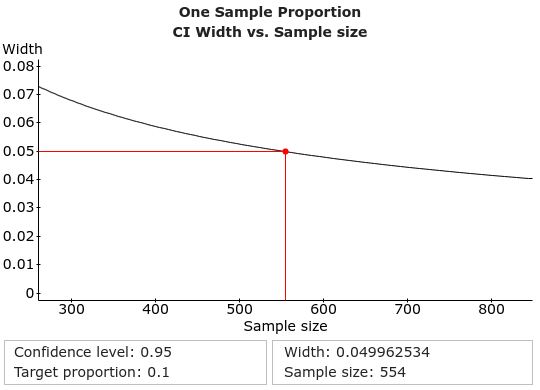
\includegraphics[width=4in]{images/grp08_Q1_a}

\newpage
\item Genetic tests are conducted on a sample of 65 redheads and it is found that 11 of them have the gene. Construct a confidence interval at a 95\% level of confidence. What conclusions can be drawn from the confidence interval?\\
\bigskip
$\ds\bv{\hat p = \frac{11}{65} = 0.169}$\\
\medskip
$\ds \bv{CI = \hat p \pm z_{\alpha/2} \times \sqrt{\frac{\hat p \times (1-\hat p)}{n} } = 0.169 \pm 1.96 \times \sqrt{\frac{0.169 \times 0.831}{65}}}$\\ \medskip
$\ds\bv{\qquad = 0.169 \pm 1.96 \times0.0465 = .0169 \pm 0.091 = (0.078, \, 0.260)}$\\
\bigskip
\bt{10\% is contained in the confidence interval. There is \emph{not} evidence that the gene occurs at a greater rate among redheads.}
\vspace{0.5in}

\item What are the null and alternative hypotheses for a test on this claim? Is this a one-sided or two-sided test? Is the claim represented by the null or alternative hypothesis?\\ \medskip
$\bv{H_0: p = 0.1}$\\
$\bv{H_a: p > 0.1}$\\
\bt{This is a one-sided test.}\\
\bt{The claim is represented by the alternative hypothesis.}
\vspace{.5in}

\end{enumalpha}



\newpage
\paragraph{2} Suppose the mean age of Metro State students is 32 years old with a standard deviation of 5.5. For a research project a stats student wants to examine the idea that students who take statistics classes are the same age as other Metro students. 
\begin{enumalpha}
\item What sample size is required to determine the mean age of stats students within plus or minus 3 years at a 99\% confidence level?\\
\medskip
\bt{\emph{By hand:}}\\
$\bv{\alpha = 0.01, \quad z_{\alpha/2} = 2.58}$\\
$\bv{ME = 3}$\\
$\bv{s = 5.5}$\\ \bigskip
$\ds \bv{n = \Paren{\frac{s \times z_{\alpha/2}}{ME}}^2 = \Paren{\frac{5.5 \times 2.58}{3}}^2 = 22.37 \implies 23}$\\
\vspace{0.5in}
\bt{\emph{From StatCrunch:}}\\
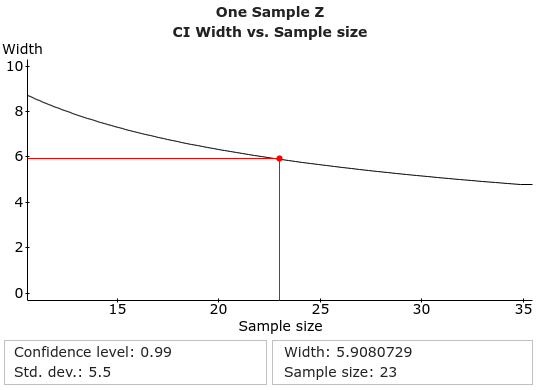
\includegraphics[width=4in]{images/grp08_Q2_a}

\newpage
\item A random sample of 25 statistics students has a mean age of 35.4 with a standard deviation of 4.6. Construct a confidence interval at a 99\% level of confidence. What conclusions can be drawn from the confidence interval?\\
\bigskip
\bt{\emph{By hand (normal approximation):}}\\
$\ds \bv{CI = \bar x \pm \frac{z_{\alpha/2} \times s}{\sqrt{n} } = 35.4 \pm \frac{2.58 \times 4.6}{5} = 35.6 \pm 2.37 = (33.23, \, 37.97)}$\\
\medskip
\bt{\emph{From StatCrunch (T Stats):}}\\
$\ds \bv{CI = (32.83, 37.97)}$\\
\bigskip
\bt{32 is not contained in the confidence interval. There is evidence stats students are older than Metro State students in general.}
\vspace{0.5in}

\item What are the null and alternative hypotheses for a test on this claim? Is this a one-sided or two-sided test? Is the claim represented by the null or alternative hypothesis?\\
\medskip
$\bv{H_0: \mu = 32}$\\
$\bv{H_a: \mu \ne 32}$\\
\bt{This is a two-sided test.}\\
\bt{The claim is represented by the null hypothesis.}
\vspace{.5in}

\end{enumalpha}

\newpage
\paragraph{3} The data file ``bears.csv" on D2L contains measurements of a random sample of bears from a national park. Park officials are concerned that the bear population is underweight and thus not prepared for the long winter. A healthy bear population has a mean weight of 200 lbs.
\begin{enumalpha}
\item A small pilot study the previous year determined the standard deviation for the weight of bears was about 100 lbs. What sample size is required to determine the mean weight of bears within plus or minus 30 lbs. at a 95\% confidence level?\\
\medskip
\bt{\emph{By hand:}}\\
$\bv{\alpha = 0.05, \quad z_{\alpha/2} = 1.96}$\\
$\bv{ME = 30}$\\
$\bv{s = 100}$\\ \bigskip
$\ds \bv{n = \Paren{\frac{s \times z_{\alpha/2}}{ME}}^2 = \Paren{\frac{100 \times 1.96}{30}}^2 = 42.68 \implies 43}$\\
\vspace{0.5in}
\bt{\emph{From StatCrunch:}}\\
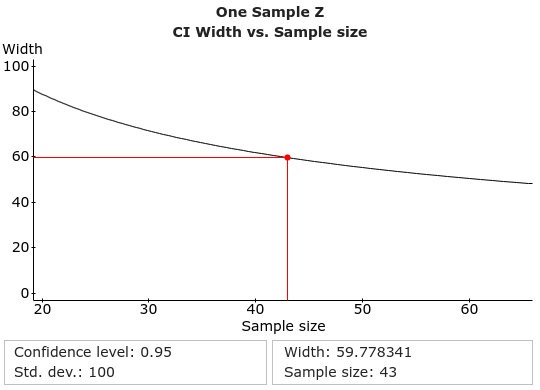
\includegraphics[width=4in]{images/grp08_Q3_a}

\newpage
\item Using the data from the ``bears.csv" construct a 95\% confidence interval.  What conclusions can be drawn from the confidence interval?\\
\bigskip
\bt{\emph{From StatCrunch (T Stats):}}\\
$\ds \bv{CI = (149.64, 216.13)}$\\

\bigskip
\bt{200 is contained in the confidence interval. There is no evidence that the bears are underweight.}
\vspace{0.5in}


\item What are the null and alternative hypotheses for a test on this claim? Is this a one-sided or two-sided test? Is the claim represented by the null or alternative hypothesis?\\
\medskip
$\bv{H_0: \mu = 200}$\\
$\bv{H_a: \mu < 200}$\\
\bt{This is a one-sided test.}\\
\bt{The claim is represented by the alternative hypothesis.}
\vspace{.5in}
\end{enumalpha}



\end{flushleft}
\end{document}